\documentclass[10pt,a4paper]{article}
\usepackage[top=1.5cm, bottom=1.5cm, left=1.6cm, right=1.6cm, headheight=14pt, footskip=18pt]{geometry}
\usepackage[utf8]{inputenc}
\usepackage{amsmath,amsfonts,amssymb}
\usepackage{graphicx}
\usepackage{tikz}
\usepackage{circuitikz}
\usetikzlibrary{calc,patterns}
\usepackage[most]{tcolorbox}
\usepackage{enumitem}
\usepackage{fancyhdr}
\usepackage{booktabs}
\usepackage{tabularx}
\usepackage{colortbl}
\usepackage{hyperref}

% --- Palet Warna Resmi UNIB ---
\definecolor{unibblue}{RGB}{0, 32, 96}
\definecolor{unibgold}{RGB}{197, 160, 89}
\definecolor{unibgreen}{RGB}{34, 112, 60}
\definecolor{boxbg}{RGB}{248, 250, 253}
\definecolor{linegray}{RGB}{210, 215, 225}

% --- Pengaturan Header & Footer ---
\pagestyle{fancy}
\fancyhf{}
\lhead{\footnotesize\textbf{\color{unibblue}Universitas Bengkulu} \textbar\ Program Studi S1 Teknik Elektro}
\rhead{\footnotesize\color{gray}Persamaan Diferensial (Genap 2026)}
\lfoot{\footnotesize\color{gray}LKM OBE \textbar\ \textbf{Video}: \url{https://youtu.be/J4XziBcVtfk} \textbar\ \href{https://www.youtube.com/playlist?list=PLS5oOZWXZeTw}{\color{unibblue}\textbf{Playlist}}}
\cfoot{\footnotesize\color{gray}Hal. \thepage\ dari 2}
\rfoot{\footnotesize\color{unibblue}\textbf{Minggu 15: Polinomial Legendre \& 4 Persamaa...}}
\renewcommand{\headrulewidth}{0.6pt}
\renewcommand{\footrulewidth}{0.4pt}

% --- Custom Box untuk Lembar Jawab ---
\newtcolorbox{answerbox}[1]{%
  colback=white,
  colframe=unibblue!70!black,
  coltitle=white,
  fonttitle=\bfseries\scriptsize,
  colbacktitle=unibblue,
  title={#1},
  arc=2pt,
  left=5pt,right=5pt,top=3pt,bottom=3pt,
  boxrule=0.6pt
}

\begin{document}

% ==================== HALAMAN 1 ====================
\noindent\begin{minipage}[c]{0.68\textwidth}%
  {\large\textbf{\color{unibblue}LEMBAR KERJA MAHASISWA (LKM)}}\\[1mm]
  {\normalsize\textbf{Mata Kuliah: Persamaan Diferensial (2 SKS)}}\\[0.5mm]
  {\small\textbf{Topik Minggu 15:} Polinomial Legendre \& 4 Persamaan Maxwell Diferensial}%
\end{minipage}%
\hfill%
\begin{minipage}[c]{0.30\textwidth}%
  \begin{tcolorbox}[colback=unibblue!5,colframe=unibblue,boxrule=0.6pt,arc=2pt,left=4pt,right=4pt,top=2pt,bottom=2pt]
    \scriptsize
    \textbf{Nama:} \dotfill\\[1.2mm]
    \textbf{NPM:} \dotfill\\[1.2mm]
    \textbf{Kelas/Klp:} \dotfill\\[1.2mm]
    \textbf{Nilai Final:} \hfill \textbf{/ 100}
  \end{tcolorbox}%
\end{minipage}\par

\vspace{1.5mm}

% Kotak Sub-CPMK & Pedoman
\begin{tcolorbox}[colback=boxbg,colframe=unibgold!90!black,boxrule=0.6pt,arc=2pt,left=5pt,right=5pt,top=3pt,bottom=3pt,title=\textbf{\scriptsize Capaian Pembelajaran (Sub-CPMK 15) \& Pedoman Evaluasi OBE}]
  \scriptsize
  \textbf{Sub-CPMK 15:} Mahasiswa mampu memecahkan Persamaan Diferensial Legendre dalam koordinat bola, menguasai 4 Persamaan Maxwell diferensial/integral, serta menyintesis kurikulum menuju medan elektromagnetika.\\
  \textbf{Video Panduan (YouTube):} \url{https://youtu.be/J4XziBcVtfk} \hfill \textbf{Playlist:} \href{https://www.youtube.com/playlist?list=PLS5oOZWXZeTw}{\color{unibblue}\textbf{bit.ly/pd-unib-playlist}}\\\textbf{Alokasi Waktu:} 50--60 Menit \quad\textbar\quad \textbf{Model:} Kolaboratif / Mandiri Terstruktur \quad\textbar\quad \textbf{Bahasa Komputasi:} Julia 1.12+
\end{tcolorbox}

\vspace{1mm}

% Soal C1
\noindent\textbf{1. (C1 - Mengingat \textbar\ Bobot: 10 Poin)}\par\vspace{0.5mm}
{\footnotesize Tuliskan bentuk baku Persamaan Diferensial Legendre: $(1-x^2)y'' - 2x y' + n(n+1)y = 0$, serta sebutkan fungsi ortogonal Polinomial Legendre berorde nol hingga dua: $P_0(x)$, $P_1(x)$, dan $P_2(x)$.}
\begin{answerbox}{Ruang Pengerjaan C1 (Persamaan Legendre \& Polinomial Tiga Orde Pertama)}
  \vspace{2.0cm}
\end{answerbox}

\vspace{1mm}

% Soal C2
\noindent\textbf{2. (C2 - Memahami \textbar\ Bobot: 15 Poin)}\par\vspace{0.5mm}
{\footnotesize Tuliskan 4 Persamaan Maxwell dalam bentuk diferensial di ruang bebas, dan jelaskan peran fisis arus pergeseran Maxwell (*displacement current* $\vec{J}_d = \frac{\partial \vec{D}}{\partial t}$) dalam menjaga kontinuitas kekekalan muatan.}
\begin{answerbox}{Ruang Pengerjaan C2 (Hukum Kekekalan Muatan \& Arus Pergeseran Maxwell)}
  \vspace{2.1cm}
\end{answerbox}

\vspace{1mm}

% Soal C3
\noindent\textbf{3. (C3 - Menerapkan \textbar\ Bobot: 20 Poin)}\par\vspace{0.5mm}
\noindent\begin{minipage}[t]{0.60\textwidth}%
  {\footnotesize Sebuah bola konduktor netral beradius $R$ diletakkan dalam medan listrik seragam luar $\vec{E}_0 = E_0 \hat{a}_z$. Solusi potensial elektrostatika di luar bola dinyatakan dalam deret Legendre: $V(r,\theta) = \sum_{n=0}^\infty \left( A_n r^n + \frac{B_n}{r^{n+1}} \right) P_n(\cos\theta)$. Turunkan solusi eksak untuk $V(r,\theta)$ dengan menerapkan syarat batas pada $r=R$ dan $r \to \infty$.}%
\end{minipage}%
\hfill%
\begin{minipage}[t]{0.37\textwidth}%
  \centering
  \resizebox{0.95\linewidth}{!}{%
  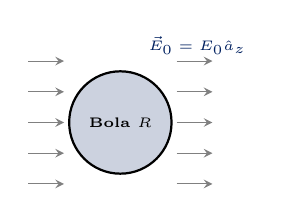
\begin{tikzpicture}[scale=0.65]
    \draw[fill=unibblue!20, thick] (0,0) circle (1.0);
    \node at (0,0) [font=\tiny\bfseries] {Bola $R$};
    \foreach \y in {-1.2, -0.6, 0, 0.6, 1.2} {
      \draw[->, >=stealth, thin, gray] (-1.8,\y) -- (-1.1,\y);
      \draw[->, >=stealth, thin, gray] (1.1,\y) -- (1.8,\y);
    }
    \node at (1.5,1.5) [font=\tiny\bfseries, unibblue] {$\vec{E}_0 = E_0 \hat{a}_z$};
  \end{tikzpicture}%
  }%
\end{minipage}\par\vspace{1mm}
\begin{answerbox}{Ruang Pengerjaan C3 (Penurunan Solusi Potensial Bola Konduktor)}
  \vspace{2.8cm}
\end{answerbox}

\newpage
% ==================== HALAMAN 2 ====================

% Soal C4
\noindent\textbf{4. (C4 - Menganalisis \textbar\ Bobot: 20 Poin)}\par\vspace{0.5mm}
{\footnotesize Analisis penurunan persamaan gelombang elektromagnetik 3D: Terapkan operasi kurva rotor ($\nabla \times (\nabla \times \vec{E})$) pada Hukum Faraday dan Hukum Ampere-Maxwell di ruang bebas muatan. Buktikan bahwa gelombang merambat dengan kecepatan $c = \frac{1}{\sqrt{\mu_0 \epsilon_0}} \approx 3 \times 10^8\text{ m/s}$!}
\begin{answerbox}{Ruang Pengerjaan C4 (Pembuktian Gelombang EM 3D \& Kecepatan Cahaya Maxwell)}
  \vspace{3.8cm}
\end{answerbox}

\vspace{1.5mm}

% Soal C5
\noindent\textbf{5. (C5 - Mengevaluasi \textbar\ Bobot: 20 Poin)}\par\vspace{0.5mm}
{\footnotesize Evaluasi Vektor Poynting $\vec{S} = \vec{E} \times \vec{H}$: Hitung densitas daya radiasi elektromagnetik rata-rata di bawah saluran udara tegangan ekstra tinggi (SUTET 500 kV PLN). Evaluasi apakah nilai densitas fluks magnetik dan medan listrik berada dalam ambang batas aman paparan publik \textbf{IEEE Std C95.1}.}
\begin{answerbox}{Ruang Pengerjaan C5 (Evaluasi Rapat Daya Poynting \& Standar Paparan SUTET IEEE C95.1)}
  \vspace{3.8cm}
\end{answerbox}

\vspace{1.5mm}

% Soal C6
\noindent\textbf{6. (C6 - Merancang \& Komputasi Julia \textbar\ Bobot: 15 Poin)}\par\vspace{0.5mm}
{\footnotesize Rancang skrip program ilmiah berbasis \textbf{Julia} untuk memvisualisasikan garis gaya medan listrik dipol bola hasil turunan Soal 3 menggunakan pustaka \texttt{Plots.jl}. Tuliskan algoritma perhitungan komponen medan radial $E_r(r,\theta)$ dan transversal $E_\theta(r,\theta)$.}
\begin{answerbox}{Ruang Pengerjaan C6 (Skrip Plotting Vektor Medan Dipol Bola Maxwell Julia)}
  \vspace{3.8cm}
\end{answerbox}

\vspace{1.5mm}

% Tabel Rekapitulasi Skor OBE & Tanda Tangan
\noindent\begin{minipage}[b]{0.65\textwidth}%
  \centering
  \scriptsize
  \begin{tabular}{|c|c|c|c|c|c|c|}
    \hline
    \rowcolor{unibblue}
    \textbf{\color{white}C1} & \textbf{\color{white}C2} & \textbf{\color{white}C3} & \textbf{\color{white}C4} & \textbf{\color{white}C5} & \textbf{\color{white}C6} & \textbf{\color{white}Total} \\
    \rowcolor{unibblue!10}
    10 Pts & 15 Pts & 20 Pts & 20 Pts & 20 Pts & 15 Pts & 100 Pts \\
    \hline
    & & & & & & \\[2.5mm]
    \hline
  \end{tabular}%
\end{minipage}%
\hfill%
\begin{minipage}[b]{0.32\textwidth}%
  \centering
  \scriptsize
  \textbf{Verifikasi Dosen / Asisten:}\\[5mm]
  (\dotfill)
\end{minipage}\par

\end{document}
